
%(BEGIN_QUESTION)
% Copyright 2011, Tony R. Kuphaldt, released under the Creative Commons Attribution License (v 1.0)
% This means you may do almost anything with this work of mine, so long as you give me proper credit

In this biogas generation system, cow manure is used as a feedstock to produce methane gas (CH$_{4}$), which is then used to fuel an engine to turn a generator and make electricity.  The waste heat from the engine is used to maintain the cascaded digesters (``reactors'' R-101 and R-102) at optimal temperatures for anaerobic bacteria to digest the manure and produce biogas (approximately 105 $^{o}$F):

$$\includegraphics[width=15.5cm]{i03526x01.eps}$$

LIC-56 registers a manure level of 3 feet 10 inches, while the operator's manual gauge reading is only 3 feet 7 inches.  The calibrated range of LT-56 is 0 to 4 feet.  Your first step is to measure current in the cable connecting LT-56 and LIC-56, and there your digital multimeter (DMM) registers 19.33 mA.

\vskip 10pt

Based on this information, determine at least two potential problems in this system.  Also, determine whether or not a hydrostatic (DP) level transmitter would be suitable for measuring manure level in R-102.

\underbar{file i03526}
%(END_QUESTION)





%(BEGIN_ANSWER)

The current value agrees with the indication at LIC-56, and so the problem is not with LIC-56.  This leaves the transmitter (miscalibrated, plugged impulse line), a change in process density (assuming a hydrostatic DP transmitter) or the operator's manual measurement of manure level.

\vskip 10pt

Hydrostatic (DP-based) level measurement is appropriate for R-102, assuming either remote seal(s) or purging.  Otherwise, solids in the manure will surely plug up the transmitter's impulse line(s) over time.

%(END_ANSWER)





%(BEGIN_NOTES)

\filbreak \vskip 20pt \vbox{\hrule \hbox{\strut \vrule{} {\bf Virtual Troubleshooting} \vrule} \hrule}

\noindent
{\bf Predicting the effect of a given fault:} present each of the following faults to the students, one at a time, having them comment on all the effects each fault would produce.

\begin{itemize}
\item{} 
\item{} 
\item{} 
\end{itemize}


\vskip 10pt


\noindent
{\bf Identifying possible/impossible faults:} present symptoms to the students and then have them determine whether or not a series of suggested faults could account for all the symptoms, explaining {\it why} or {\it why not} for each proposed fault:

\begin{itemize}
\item{} Symptom: {\it }
\item{}  -- {\bf Yes/No}
\item{}  -- {\bf Yes/No}
\item{}  -- {\bf Yes/No}
\end{itemize}


\vskip 10pt


\noindent
{\bf Determining the utility of given diagnostic tests:} present symptoms to the students and then propose the following diagnostic tests one by one.  Students rate the value of each test, determining whether or not it would give useful information (i.e. tell us something we don't already know).  Students determine what different results for each test would indicate about the fault, if anything:

\begin{itemize}
\item{} Symptom: {\it }
\item{}  -- {\bf Yes/No}
\item{}  -- {\bf Yes/No}
\end{itemize}


\vskip 10pt


\noindent
{\bf Diagnosing a fault based on given symptoms:} imagine the LT-55 fails with a 21.5 mA signal in this system (don't reveal the fault to students!).  Present the operator's observation(s) to the students, have them consider possible faults and diagnostic strategies, and then tell them the results of tests they propose based on the following symptoms, until they have properly identified the nature and location of the fault:

\begin{itemize}
\item{} {\it Operator complains about gas production being abnormally low}
\item{} LT-55 registers 109\%
\item{} LIC-55 output 0\% (LV-55a full open, LV-55b full shut)
\item{} TT-41 reads ambient temp (58 deg) while setpoint of TIC-41 is 100 deg
\item{} LIC-56 reads right at setpoint
\item{} TIC-48 reads right at setpoint, TV-48 valve at 87\% open through exchanger (normally 45\% open)
\item{} TIC-43 reads right at setpoint, E-49 fan at 70\% speed (normally at 30\% speed)
\end{itemize}





%INDEX% Basics, control loop troubleshooting
%INDEX% Process: anaerobic digester (manure)

%(END_NOTES)


